\documentclass[12pt]{beamer}

\usetheme{Boadilla}
\usecolortheme{default}

\usepackage[utf8]{inputenc}
\usepackage[T1]{fontenc}
\usepackage[brazil]{babel}
\usepackage{amsmath, amssymb}
\usepackage{booktabs}
\usepackage{graphicx}

\title{O que acontece quando capturamos uma população?}
\subtitle{Introduzindo captura no modelo logístico}
\author{Modelagem Matemática}
\institute{Matemática Aplicada}
\date{Aula 03}

\begin{document}

% ── CAPA ──────────────────────────────────────────
\begin{frame}
  \titlepage
\end{frame}

% ══════════════════════════════════════════════════
\section{Ponte com a aula anterior}
% ══════════════════════════════════════════════════

\begin{frame}{Onde estamos}

  Na aula anterior construímos dois modelos e ficamos com uma pergunta aberta:

  \bigskip
  \begin{block}{Modelo logístico — Aula 02}
    \[
      \frac{dN}{dt} = rN\!\left(1 - \frac{N}{K}\right)
    \]
    Três hipóteses: população fechada, dependência de densidade linear,
    sem perturbação externa.
  \end{block}

  \bigskip
  \begin{alertblock}{Pergunta em aberto}
    O que os dados reais dizem sobre $r$ e $K$?\\
    E se houver retirada contínua de indivíduos --- pesca, caça, colheita?
  \end{alertblock}

\end{frame}

% ══════════════════════════════════════════════════
\section{Bloco 1 — Problema concreto}
% ══════════════════════════════════════════════════

\begin{frame}{Um estoque que encolheu}

  \begin{center}
    \includegraphics[width=0.80\textwidth]{cpue_compact.pdf}
  \end{center}

  \smallskip
  {\small Fonte: SCPESCA/MS --- Catella et al., Boletins Embrapa Pantanal (1994--2017)}

  \bigskip
  \begin{alertblock}{Pergunta}
    A CPUE (captura por unidade de esforço) do pintado caiu de
    $\approx 55$ para $\approx 23\;\text{t}/10\text{k}$ pescadores em 23 anos
    --- com esforço relativamente estável.
    O modelo logístico sozinho explica isso?
  \end{alertblock}

\end{frame}

% ──────────────────────────────────────────────────
\begin{frame}{O modelo logístico não tem retirada}

  O logístico descreve uma população \textbf{sem perturbação externa}:

  \[
    \frac{dN}{dt} = rN\!\left(1 - \frac{N}{K}\right)
  \]

  \bigskip
  Sem captura, o modelo prediz que $N \to K$.\\
  Mas os dados mostram declínio contínuo mesmo sem crescimento do esforço.

  \bigskip
  \begin{exampleblock}{Conclusão}
    O logístico precisa de um novo termo: a \textbf{retirada contínua}.\\
    A questão é: como representá-la?
  \end{exampleblock}

\end{frame}

% ══════════════════════════════════════════════════
\section{Bloco 2 — Construindo o modelo}
% ══════════════════════════════════════════════════

\begin{frame}{Captura como processo que diminui $N$}

  Voltemos à identidade contábil da Aula 02:

  \[
    \Delta N = B - D + I - E
  \]

  \bigskip
  Com população fechada ($I = E = 0$), tínhamos $\Delta N = B - D$.

  \bigskip
  A captura $H$ (do inglês \emph{harvest}) é um novo processo
  que \textbf{diminui} $N$:

  \[
    \frac{dN}{dt} = \underbrace{B - D}_{\text{logístico}} - \underbrace{H}_{\text{captura}}
  \]

  \bigskip
  \begin{alertblock}{Pergunta}
    Do que $H$ depende?
    Quais hipóteses podemos fazer sobre a captura?
  \end{alertblock}

\end{frame}

% ──────────────────────────────────────────────────
\begin{frame}{Hipótese 4 --- Captura constante}

  \begin{exampleblock}{Hipótese explícita}
    A retirada de indivíduos por unidade de tempo é constante:
    $H = \text{cte}$, independente de $N$, do tempo ou do esforço.
  \end{exampleblock}

  \bigskip
  \textbf{Quando é razoável?}
  \begin{itemize}
    \item Cota de captura fixada por política pública (e.g.\ cota anual de pesca)
    \item Colheita agrícola com quantidade predefinida por contrato
    \item Caça com licença de número fixo de abates
  \end{itemize}

  \bigskip
  \begin{block}{Atenção}
    \textbf{Custo:} ignora que capturas menores são mais difíceis quando o
    estoque é pequeno --- o esforço real aumenta para manter $H$ constante.\\
    \textbf{Ganho:} modelo analiticamente tratável; permite análise qualitativa completa.
  \end{block}

\end{frame}

% ──────────────────────────────────────────────────
\begin{frame}{O modelo com captura constante}

  Substituindo $H = \text{cte}$ no logístico:

  \[
    \boxed{\frac{dN}{dt} = rN\!\left(1 - \frac{N}{K}\right) - H}
  \]

  \bigskip
  Cada símbolo é uma \textbf{hipótese explícita}:

  \bigskip
  \begin{itemize}
    \item $N$ --- abundância (o que queremos entender)
    \item $r$ --- taxa intrínseca de crescimento (sem limitação, sem captura)
    \item $K$ --- capacidade de suporte (limite imposto pelo ambiente)
    \item $H$ --- captura por unidade de tempo (\textbf{nova hipótese}: constante)
  \end{itemize}

\end{frame}

% ══════════════════════════════════════════════════
\section{Bloco 3 — Análise qualitativa}
% ══════════════════════════════════════════════════

\begin{frame}{Como analisar sem resolver a EDO?}

  Equilíbrios são os valores de $N$ onde $\dfrac{dN}{dt} = 0$:

  \[
    rN\!\left(1 - \frac{N}{K}\right) - H = 0
    \quad\Longleftrightarrow\quad
    f(N) = H
  \]

  onde $f(N) = rN(1 - N/K)$ é a \textbf{curva de crescimento logístico}.

  \bigskip
  \begin{block}{Estratégia gráfica}
    Plotar $f(N)$ e a linha horizontal $H$ no mesmo gráfico.\\
    As \textbf{interseções} são os equilíbrios.\\
    O \textbf{sinal} de $f(N) - H$ indica se $N$ cresce ou decresce.
  \end{block}

\end{frame}

% ──────────────────────────────────────────────────
\begin{frame}{Diagrama de fase --- três regimes}

  \begin{center}
    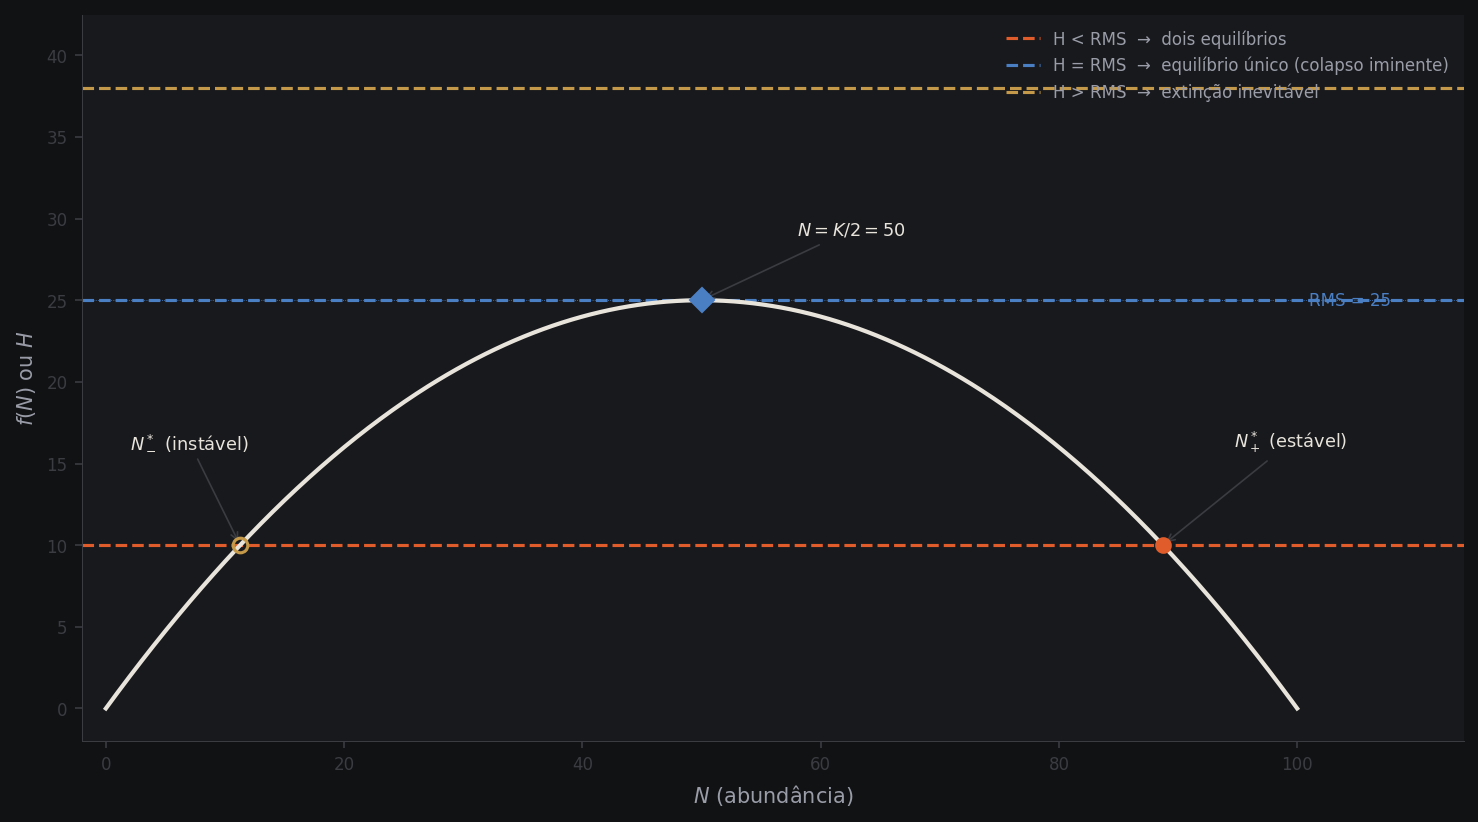
\includegraphics[width=\textwidth]{diagrama_captura.pdf}
  \end{center}

  {\small $r = 1{,}0$;\; $K = 100$;\; RMS $= rK/4 = 25$}

\end{frame}

% ──────────────────────────────────────────────────
\begin{frame}{Interpretando os equilíbrios}

  Quando $H < \text{RMS}$ existem \textbf{dois equilíbrios}:

  \bigskip
  \begin{columns}[T]
    \column{0.48\textwidth}
      \begin{exampleblock}{$N^*_+$ --- equilíbrio alto (estável)}
        \begin{itemize}
          \item Crescimento logístico supera a captura
          \item Se perturbado, $N$ retorna a $N^*_+$
          \item \textbf{Manejo sustentável possível}
        \end{itemize}
      \end{exampleblock}
    \column{0.48\textwidth}
      \begin{alertblock}{$N^*_-$ --- equilíbrio baixo (instável)}
        \begin{itemize}
          \item Qualquer perturbação para baixo:
            $N \to 0$ (extinção)
          \item Qualquer perturbação para cima:
            $N \to N^*_+$
          \item \textbf{Limiar de colapso}
        \end{itemize}
      \end{alertblock}
  \end{columns}

  \bigskip
  \begin{block}{Intuição}
    O equilíbrio instável $N^*_-$ é o ``ponto de sem retorno'':
    abaixo dele, a captura supera o crescimento para sempre.
  \end{block}

\end{frame}

% ══════════════════════════════════════════════════
\section{Bloco 4 — Quebrando a hipótese}
% ══════════════════════════════════════════════════

\begin{frame}{O que acontece quando $H$ cresce?}

  À medida que $H$ aumenta, os dois equilíbrios se aproximam:

  \bigskip
  \begin{itemize}
    \item $N^*_+$ desce (estoque sustentável encolhe)
    \item $N^*_-$ sobe (limiar de colapso sobe)
    \item Quando $H = rK/4$: os dois se fundem em $N = K/2$
  \end{itemize}

  \bigskip
  \begin{exampleblock}{Definição — Rendimento Máximo Sustentável (RMS)}
    \[
      H_{\max} = \frac{rK}{4}
      \qquad \text{atingido em } N^* = \frac{K}{2}
    \]
    É o maior valor de $H$ para o qual o modelo ainda admite equilíbrio estável.
  \end{exampleblock}

  \bigskip
  \begin{alertblock}{Pergunta}
    O que acontece quando $H > H_{\max}$?
  \end{alertblock}

\end{frame}

% ──────────────────────────────────────────────────
\begin{frame}{Quando $H > \text{RMS}$: extinção inevitável}

  Se $H > rK/4$, a linha $H$ fica \emph{acima} de $f(N)$ para todo $N > 0$:

  \[
    \frac{dN}{dt} = f(N) - H < 0 \quad \text{para todo } N > 0
  \]

  \bigskip
  Não importa o tamanho inicial da população:
  $N(t) \to 0$ em tempo finito.

  \bigskip
  \begin{block}{Ligação com os dados do Pantanal}
    A CPUE do pintado sugere declínio contínuo sem sinal de
    estabilização: o sistema pode estar operando próximo ou
    acima do RMS, no regime onde não existe equilíbrio estável.
  \end{block}

  \bigskip
  \begin{alertblock}{Atenção}
    O modelo não diz \emph{quando} a extinção ocorre ---
    apenas que ela é inevitável. Para \emph{quando}, é necessário
    resolver a EDO.
  \end{alertblock}

\end{frame}

% ══════════════════════════════════════════════════
\section{Síntese}
% ══════════════════════════════════════════════════

\begin{frame}{Síntese --- Como chegamos até aqui}

  \begin{enumerate}
    \item \textbf{Problema concreto:} CPUE do pintado cai 23 anos
      --- logístico sozinho não explica
    \bigskip
    \item \textbf{Captura na identidade contábil:}
      $\dot{N} = (B - D) - H$
    \bigskip
    \item \textbf{Hipótese 4 --- captura constante:}
      $\dot{N} = rN(1 - N/K) - H$
    \bigskip
    \item \textbf{Análise gráfica:} dois equilíbrios
      --- $N^*_+$ estável, $N^*_-$ instável (limiar)
    \bigskip
    \item \textbf{RMS:} $H_{\max} = rK/4$ ---
      acima disso, extinção inevitável
  \end{enumerate}

\end{frame}

% ──────────────────────────────────────────────────
\begin{frame}{O modelo é um argumento}

  \begin{block}{Para refletir}
    O modelo com captura constante revela uma assimetria essencial:
    a mesma captura $H$ pode ser sustentável ou destrutiva ---
    dependendo de onde $N$ está em relação a $N^*_-$.
    Monitorar a abundância é tão importante quanto monitorar a captura.
  \end{block}

  \bigskip
  \begin{exampleblock}{Próxima aula}
    A hipótese de captura constante é razoável?
    \begin{itemize}
      \item Na prática, o esforço cresce quando o estoque é abundante
        e diminui quando é escasso
      \item E se $H = qEN$, onde $E$ é o esforço e $q$ a capturabilidade?
      \item O que muda nos equilíbrios?
    \end{itemize}
  \end{exampleblock}

\end{frame}

\end{document}
